% Assignment 0 writeup skeleton for DATA 8014 (Fall 2026).
% NOTE: per course policy the writeup must be written by you, not AI.
% The figures referenced here are produced by the scripts in scripts/ and are
% read from ../outputs/figures/. Compile with: pdflatex writeup.tex
\documentclass[11pt]{article}
\usepackage[margin=1in]{geometry}
\usepackage{amsmath, amssymb}
\usepackage{graphicx}
\usepackage{hyperref}

\graphicspath{{../outputs/figures/}}

\title{DATA 8014 --- Assignment 0: Setting Up the Codebase}
\author{Your Name (Your Student ID)}
\date{Fall 2026}

\begin{document}
\maketitle

\section{Repository}
% TODO: URL of your private repository in the hku-data8014-students organization.

\section{Code Structure and Abstractions}
% TODO: briefly describe the package layout and the Trainer /
% InferenceEngine / EvalRunner abstractions, in your own words.

\section{Data: MNIST Augmentation}
\begin{figure}[h]
  \centering
  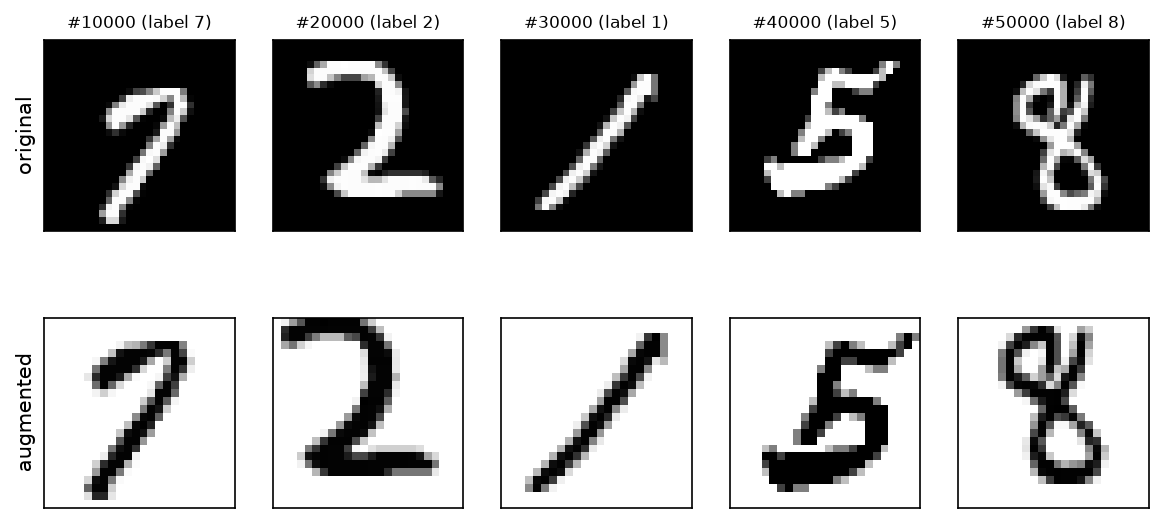
\includegraphics[width=\linewidth]{mnist_augmented_samples.png}
  \caption{TODO: explain the inversion + random-crop pipeline and comment on
  the five requested training images (positions 10{,}000--50{,}000).}
\end{figure}

\section{Training: Linear Regression on Gaussian Data}
\begin{figure}[h]
  \centering
  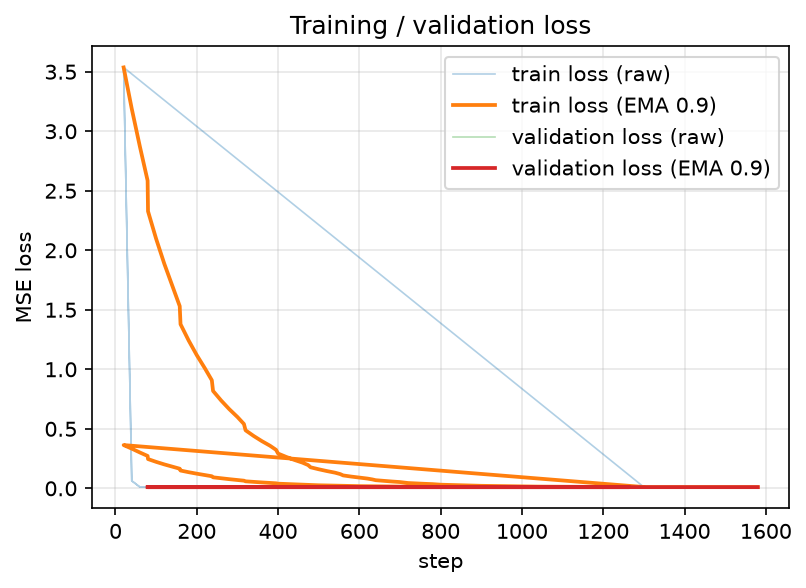
\includegraphics[width=0.48\linewidth]{train_val_loss.png}
  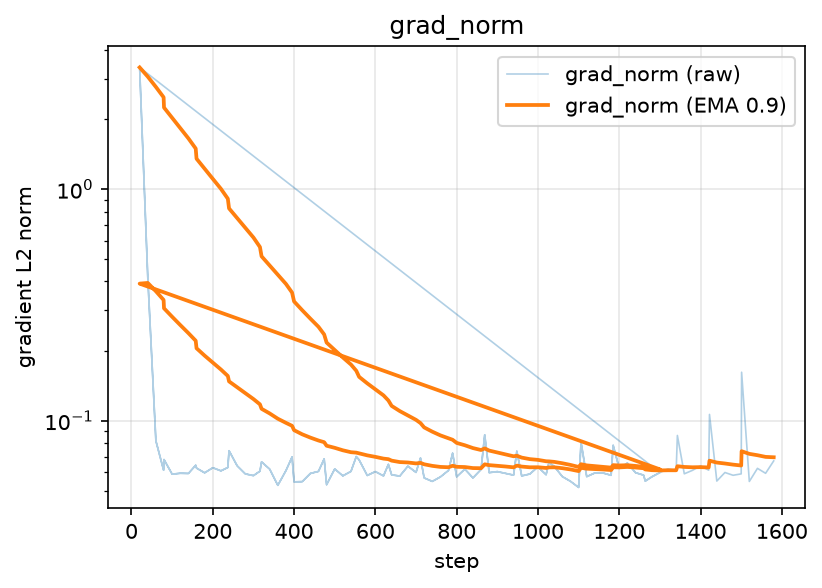
\includegraphics[width=0.48\linewidth]{train_grad_norm.png}
  \caption{TODO: train/validation loss and gradient norm.}
\end{figure}
\begin{figure}[h]
  \centering
  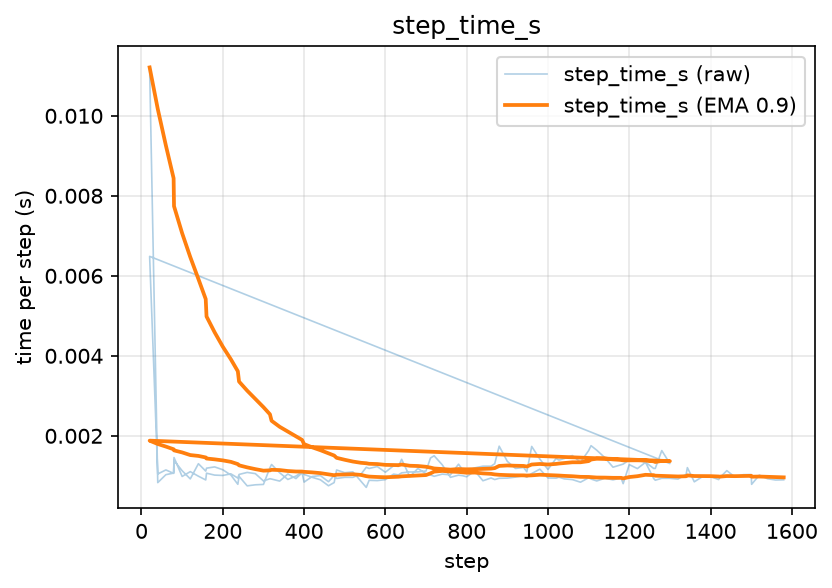
\includegraphics[width=0.48\linewidth]{train_step_time_s.png}
  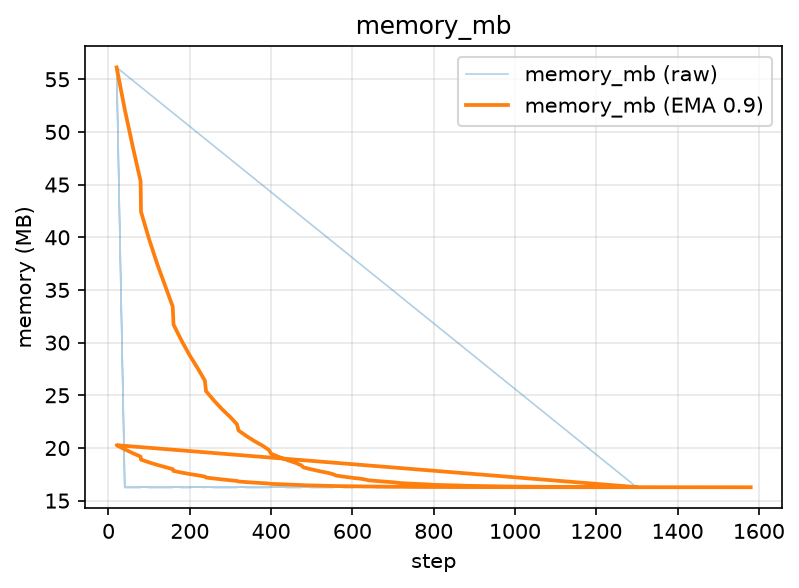
\includegraphics[width=0.48\linewidth]{train_memory_mb.png}
  \caption{TODO: time per step and memory usage.}
\end{figure}
\begin{figure}[h]
  \centering
  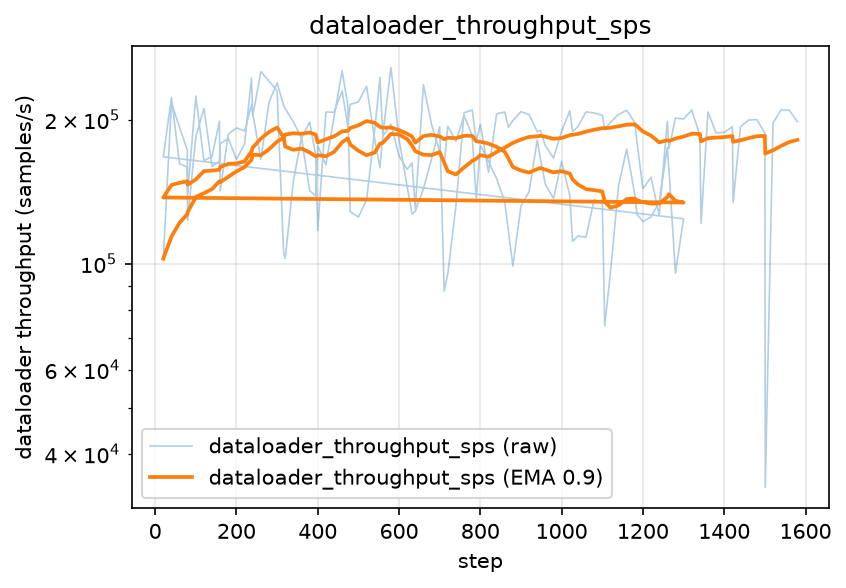
\includegraphics[width=0.48\linewidth]{train_dataloader_throughput_sps.png}
  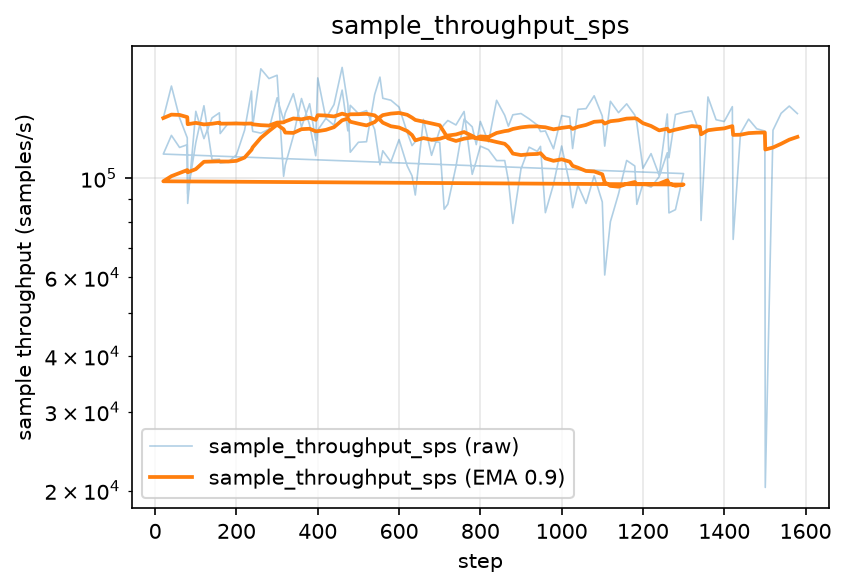
\includegraphics[width=0.48\linewidth]{train_sample_throughput_sps.png}
  \caption{TODO: dataloader and sample throughput.}
\end{figure}
\begin{figure}[h]
  \centering
  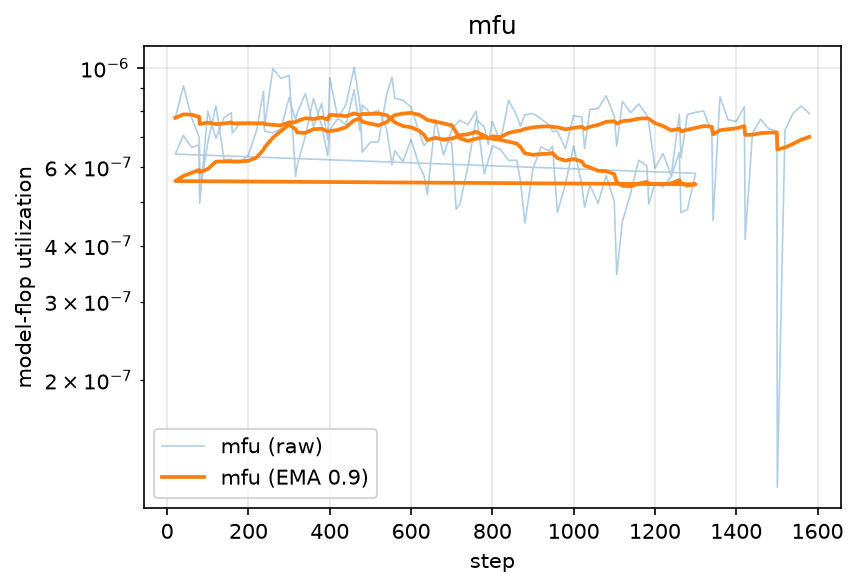
\includegraphics[width=0.48\linewidth]{train_mfu.png}
  \caption{TODO: model-flop utilization; explain why it is tiny for this
  model and how the peak was measured.}
\end{figure}

\section{Inference}
\begin{figure}[h]
  \centering
  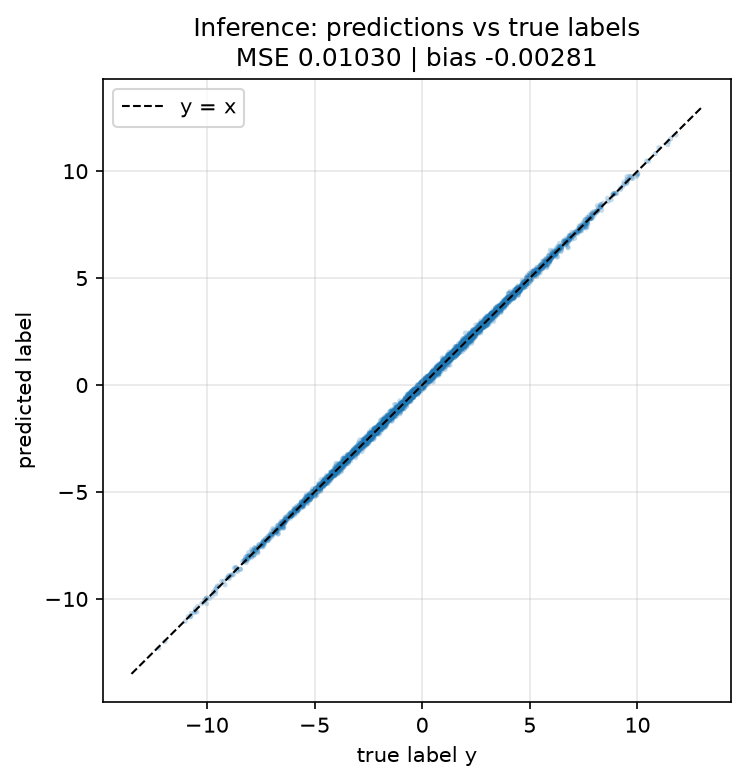
\includegraphics[width=0.6\linewidth]{inference_true_vs_pred.png}
  \caption{TODO: true labels vs predictions; comment on accuracy and bias.}
\end{figure}

\section{Evaluation}
\begin{figure}[h]
  \centering
  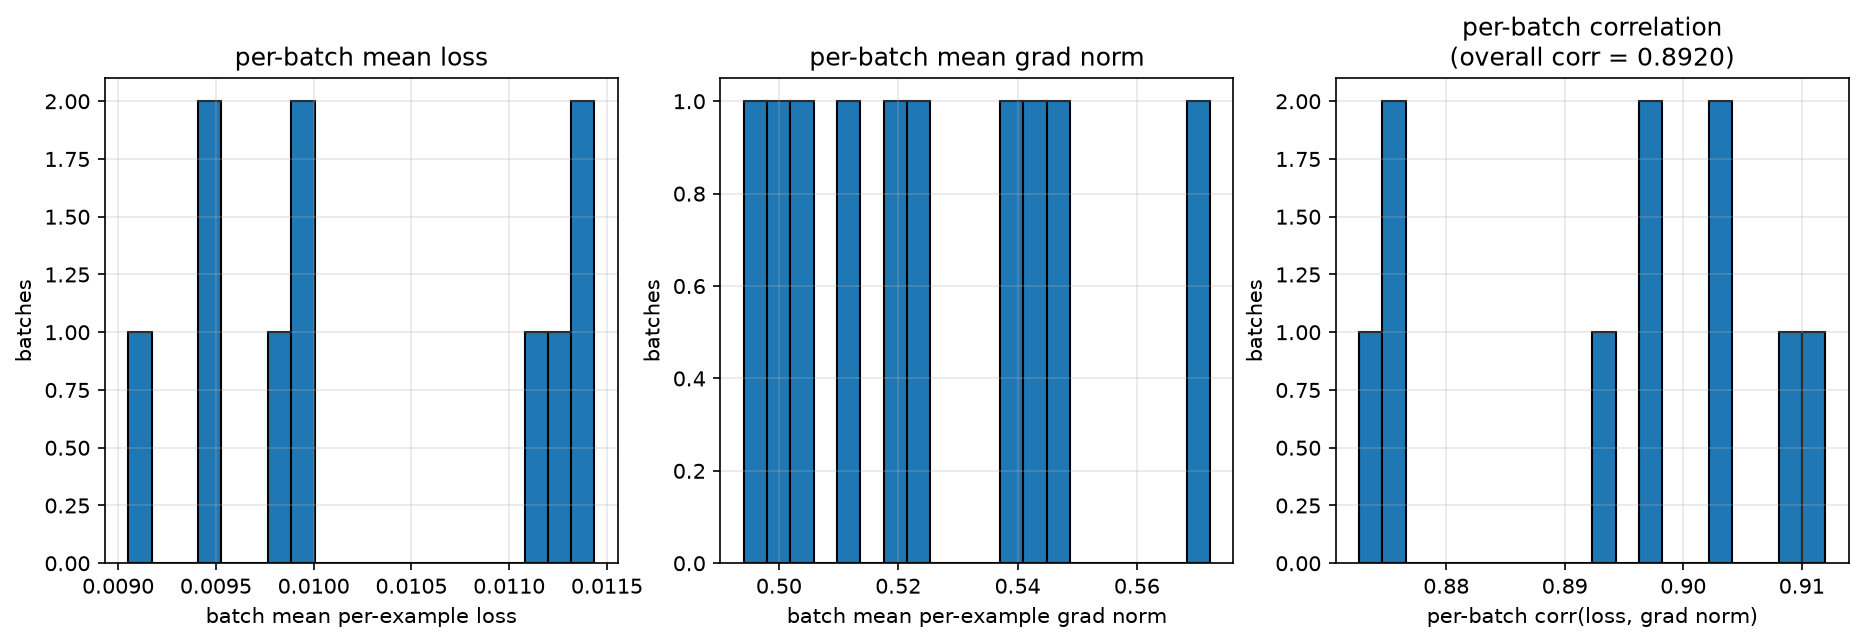
\includegraphics[width=\linewidth]{eval_batch_metric_histograms.png}
  \caption{TODO: histograms of per-batch mean loss, per-batch mean gradient
  norm, and per-batch correlation; report the overall correlation.}
\end{figure}
\begin{figure}[h]
  \centering
  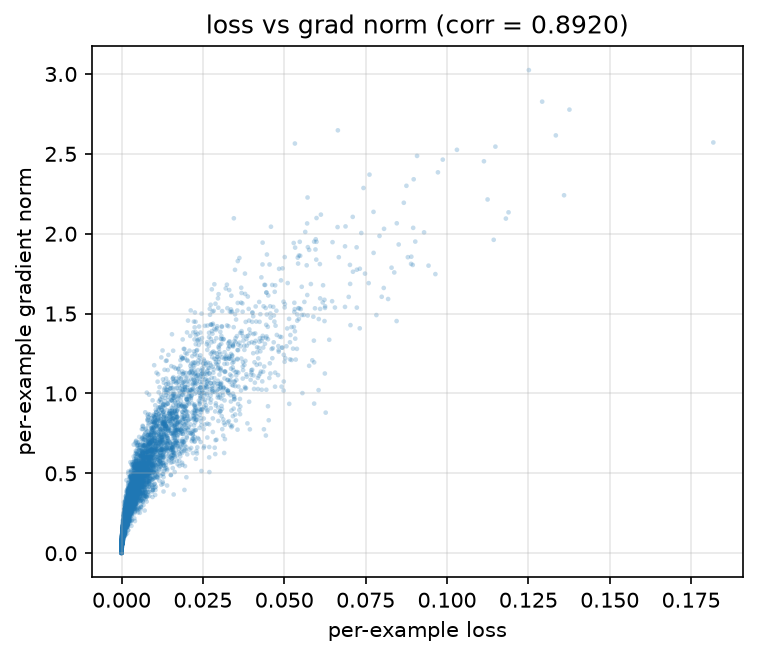
\includegraphics[width=0.6\linewidth]{eval_loss_vs_grad_norm.png}
  \caption{TODO: per-example loss vs gradient norm.}
\end{figure}

\section{AI Usage Disclosure}
% TODO: disclose where and how you used AI (models, settings, which parts),
% and confirm that you understand the outputs. Written by you, not AI.

\end{document}
